\documentclass{article}
%\usepackage[2.5cm]{geometry}
%\usepackage{fullpage}
\usepackage{graphicx}
\title{Parallel Image Processing Report}
\date{\today}
\author{Simon Richards (scr52@uclive.ac.nz)}

\begin{document}
\maketitle
\section{Introduction}
An exploration probe belonging to a Chinese mining company has returned from a
two year mission to the Orion Nebula with  approximately 10 million images which
have suffered both motion and Gaussian blur. The company has put out a tender
for the restoration of these images using the iterative and computationally
expensive Richardson-Lucy deconvolution algorithm. This report details a brief
investigation of the time and money costs for a potential bid on this contract.

\paragraph{Test Rig}
All performance metrics, unless explicitly stated otherwise, were calculated on
a Linux VM running on an AMD Deneb quad-core 3.2GHz CPU with 8 gigabytes of
memory. The effects of running the program on other systems was not explored and
it was assumed that no order-of-magnitude change could be attained. That said,
non-trivial gains could definitely be achieved by upgrading from what is now a
two year old architecture and also possibly by removing the overheads imposed by running a
virtual machine.

\section{Implementation}
A single core working with a small point spread function kernel may complete ten
iterations (enough to noticeably improve the image) on a single channel,
1024x1024 sized image in 2-10 seconds. Even at two seconds per image this would
result in the entire dataset being processed in over 230 days, a delay which may
be unacceptable to the clients. To improve on this time, a double pronged
approach to parallelism has been taken leveraging multiple core CPUs and
multiple computers in a cluster.

\subsection{Class Descriptions}
The task is split into two main classes, an IO class for reading and writing
images and a filter class capable of efficiently restoring images using the
Richardson-Lucy algorithm.

\subsubsection{ImageQueue}
The first is a producer class which
reads the input directory and pushes the names of all the image files contained in that
directory onto a stack. On request it pops a file name off the stack and reads the
data contained into a buffer using the CFITSIO library. FITS is the flexible
image transport system which is popular in scientific fields, especially
astronomy, and is used in this project mostly for the simple way it handles
double precision pixels and dynamic maximum/minimum values.

\subsubsection{DeconvFilter}
The second, and more important, class is the DeconvFilter consumer class.
This class takes a PSF and allocates all the memory space it needs on
construction so that processing a single image is done without any unnecessary
overhead. For small kernel sizes (see discussion) the algorithm is as follows:
\begin{verbatim}
FOR iteration = 1 to niter
    temp  = image*psf
    temp  = original_image / temp;
    temp  = temp*psf
    image = temp.*image
ENDFOR
\end{verbatim}
Where / is a per element division, * is the convolution operator and .* is a per
element multiply.

\subsubsection{FFT vs Direct Convolution}
For large kernels the algorithm is equivalent however slightly more involved as
convolution is achieved by performing a fast Fourier transform on both matrices,
multiplying the matrices' elements (not the same thing as matrix multiplication)
and then performing an inverse Fourier transform. The second option was not
explored past a simple implementation using the FFTW (Fastest Fourier Transform
in the West) library.

Direct convolution is $O(N^2)$ where N is the image size.
However since the point spread function may be simplified to a small kernel of
non-zero values this can be made $O(NM)$ where is M is the kernel size. This
means the algorithm quickly slows past the speed of the FFT approach
as the kernel size increases. That said, for small values of M this is still
a much faster option.

The other option being fast Fourier transforms. According to the convolution
theorem, the Fourier transform of a convolution is the pointwise product of
Fourier transforms. This algorithm is $O(NlogN)$, a much more attractive option
for large kernels and one that was implemented using the FFTW but not used or
fully tested.

\subsubsection{Further Work}
File IO times are minimal in comparison to that that of the deconvolution filter
however we do wish to shave as much time off as possible. Therefore the final
implementation of this project would see a concurrent producer-consumer model
implemented using a semaphore to ensure that a new image is always ready for the
filter thread and that the algorithm is never waiting on a disk or network
transfer. For this reason IO times are not considered in the calculations seen
in the results section.

\subsection{OpenMP}
OpenMP is an API for Fortran and C/C++ which provides a simple yet powerful
interface to both task and data parallelism. Worker threads are instantiated
cheaply and inline with as little as a single line OMP directive such as:
\begin{verbatim}
#pragma omp parallel for private(...) shared(...)
\end{verbatim}

Adding this directive to the convolution function expressed previously resulted
in an execution speed 0.90*4 (quad-core) times faster than the single
threaded implementation. The other steps of the algorithm were also parallelised
in a similar manner however as they were all O(n) the effect of doing this was
negligible.

\subsection{MPI}
Message Passing Interface is a popular standard for communication between
processes in distributed memory systems such as cluster compute set ups.

It enables easy execution and communication between processes in the cluster
which allowed the software to be converted into a distributed version with
minimal effort. The system with MPI uses a master node which is responsible for
the producer class and therefore is the node with direct access to the images.
The rest of the nodes are workers which request an image, process it, then
return it. As stated previously, the transfer times are short (theoretically
they would take ~8ms on an 8Gb/s Infiniband link) however in the final system
these transfers would be made asynchronously and buffered so that execution time
is dependent only on the deconvolution algorithm.

\subsection{Unknown Variables}
Before reading the next section it is important to note there are two unknown
factors which may influence the results.
\begin{itemize}
\item[Kernel size] The point spread function determined to be the cause of noise
on the images may be described as a rectangular matrix of any size smaller than
the image itself. When using Fourier transforms to perform convolution the size
of the kernel is irrelevant. When performing convolution manually however
increases in the kernel size result in the same increase in execution time. For
example a 7x7 sized kernel will take $49/9$ times longer to run than a 3x3. More
information will be needed from the client in order to properly estimate the
project requirements. Regardless, all execution times mentioned in this report
are for a 3x3 kernel which produced visually adequate results.
\item[Image channels] The deconvolution filter currently treats a single buffer
as one image, although it would be trivial to implement multiple buffers per
image this was not done as the concept of RGB channels is not particularly
relevant in astronomy. If the images are in fact 3 channel then all performance
values will just need to be tripled. Again, please ask the client to clarify this.
\end{itemize}

\section{Results}
As previously explained all of the following results were obtained on a 3.2GHz
quadcore running as a virtual machine. GCC compiled the program with full
optimisation (-O3), a flag which roughly halved execution time and cut the
number of instructions inside the most important loop down by almost two thirds.
The kernel dimensions were 3x3 and 10
iterations were performed on single channel images. An example output from this
is attached to this report.

The program was benchmarked by performing 1000 iterations with a total execution
time of 32.7 seconds which translates into 32.7ms per iteration or 0.327 seconds
for an image.

For ~10 million images this means the running time for a single computer is just
under 38 days. For a more reasonable time we spread the load over a number of
computers using the MPI technique described above.

In order to maximise efficiency the controller thread may be run on the same machine as a
worker, using just a single core as it is not computationally demanding. This
configuration means the execution time will be $38/(N_{computers}-0.25)seconds$.

The only constraint on MPI based systems that has not yet been considered is the
bandwidth requirement. For a typical network speed of 8Gbit/s, 128 images may be
transferred per second. Since data must be returned to the controller node this
value must be halved to 64 images processed per second. If the nodes can process
an image in 0.327 seconds then an 8GBit/s connection limits us to a maximum of
21 nodes per master. Since this value is considerably more than would be required anyway (the
entire job would finish in 1.8 days at that rate), and is an underestimate
anyway due to the switched fabric topology of Infiniband, this will not cause a
problem and was not investigated further.

\section{Recommendations}
If the PSF requires a large enough kernel to make the FFT method the faster
option then it is recommended to purchase or hire a cluster GPU instance such as
the US\$100,000 prebuilt GPU Computing Kit from HP which should be able to complete
the task within a week (although I have no data to back this up).

If not then a cheaper, cpu-heavy cluster should be bought or hired according to
figure \ref{comps-vs-time} and the client's preference.

\begin{figure}[h!]
\caption{Execution length for different sized clusters.}
\centering
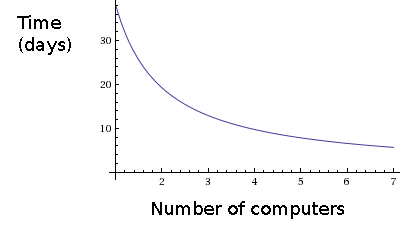
\includegraphics[width=0.5\textwidth]{comps-vs-time}
\label{comps-vs-time}
\end{figure}

All of these figures will need to be re-evaluated depending on both caveats
mentioned in the Unknown Variables section, the client's expectations for
time till completion and the number and speed of cores in the purchased or hired
computers.

\end{document}

